\documentclass[11pt,xcolor=dvipsnames,aspectratio=169]{beamer}

\mode<presentation>
{
  \useinnertheme{circles} 
  \usecolortheme[named=Black]{structure} 
  \setbeamertemplate{navigation symbols}{}
  \setbeamertemplate{footline}[page number]
  \setbeamercovered{transparent}
}

\usepackage{physcomm}

%\usepackage{adjustbox}
\usepackage[export]{adjustbox}
\usepackage{graphicx}
\usepackage{colortbl}
\usepackage{pifont}
\usepackage{amsmath}
\usepackage{scrdate,scrtime}
\usepackage{subfig}
\usepackage{verbatim}
\usepackage{booktabs}
\usepackage{rotating}
\usepackage{xspace}
\usepackage{xcolor}
\usepackage{bm}
\usepackage{pdfpages}
\usepackage{enumerate}
\usepackage{amsmath}
\usepackage{xspace}
\usepackage{ifthen}
 
%-----------------------------------------------------------------------
% custom colors 
\definecolor{EDBRed}{RGB}{220,20,60} 
\definecolor{EDBDarkBlue}{RGB}{0,0,160}
\definecolor{EDBBlue}{RGB}{0,135,189}
\definecolor{EDBGray}{RGB}{211,211,211}

%-----------------------------------------------------------------------
% text boxes 
\usepackage{tcolorbox}
%\usepackage{mdframed}

% 1- Block title (background and text)
\setbeamercolor{block title}{bg=EDBBlue!60, fg=black}
% 2- Block body (background)
\setbeamercolor{block body}{bg=EDBBlue!60}

\setbeamercolor{block title alerted}{fg=white, bg=orange}
% 2- Block body (background)
\setbeamercolor{block body alerted}{bg=orange!25}

% 1- Block title (background and text)
\setbeamercolor{block title example}{fg=white, bg=teal}
% 2- Block body (background and text)
\setbeamercolor{block body example}{bg=EDBBlue!60}

% arrows between color boxes
\usepackage{tikz}
\usetikzlibrary{arrows.meta, % for arrows style
                positioning  % for positioning of boxes
               }

%-----------------------------------------------------------------------
% backup 
\newcommand{\backupbegin}{
   \newcounter{framenumberappendix}
   \setcounter{framenumberappendix}{\value{framenumber}}
    \setbeamertemplate{footline}{
   \leavevmode%
   \hbox{%
   \begin{beamercolorbox}[wd=1.00\paperwidth,ht=0.01ex,dp=1ex,right]{} 
     {\normalsize \insertframenumber{}} \hspace{0.065\textwidth}
   \end{beamercolorbox}
   }%
   \vskip0pt%
 }
}

\newcommand{\backupend}{
   \addtocounter{framenumberappendix}{-\value{framenumber}}
   \addtocounter{framenumber}{\value{framenumberappendix}} 
}

% -----------------------------------------------------------------------
% slide layout & footnotes
\setbeamertemplate{frametitle}{ 
%\begin{centering} 
\vspace{0.03\paperheight}
{\huge \insertframetitle }
\vspace{0.01\paperheight}
\par 
%\end{centering} 
}


%\setbeamertemplate{footline}[text line]{%
%\parbox{\linewidth}{\small \vspace*{-10pt} \ \hfill \ \insertpagenumber / \inserttotalframenumber}}

\setbeamertemplate{footline}[text line]{%
\parbox{\linewidth}{\small \vspace*{-10pt} \ \hfill \ \insertframenumber / \inserttotalframenumber}}

\let\footnoterule\relax

\newcommand\blfootnote[1]{%
  \begingroup
  \renewcommand\thefootnote{}\footnote{\hspace{-30pt}\textcolor{Gray}{\tiny #1}}%
  \addtocounter{footnote}{-1}%
  \endgroup
}

% -----------------------------------------------------------------------
% itemize margins
\setlength{\leftmargini}{0.025\linewidth}
\setlength{\leftmarginii}{0.021\linewidth}

% sub-item size:
\setbeamerfont{itemize/enumerate subbody}{size=\normalsize} %to set the body size
%\setbeamertemplate{itemize subitem}{\normalsize\raise1.25pt\hbox{\donotcoloroutermaths$\blacktriangleright$}}  %to set the symbol size 
% -----------------------------------------------------------------------
\begin{document}

{
\usebackgroundtemplate{
\includegraphics[width=\paperwidth]{background/template_169_logos.pdf}}%
\begin{frame}[noframenumbering,plain]
  \begin{center}
    \setlength{\parskip}{0pt}
    \vspace{10pt}
    {\Huge\bf Deep Learning \& the Higgs Boson}\\[0.1\textheight]
    {\huge \bf Dr. Liza Mijovi\'c}
  \end{center}
\end{frame}
}

{
\usebackgroundtemplate{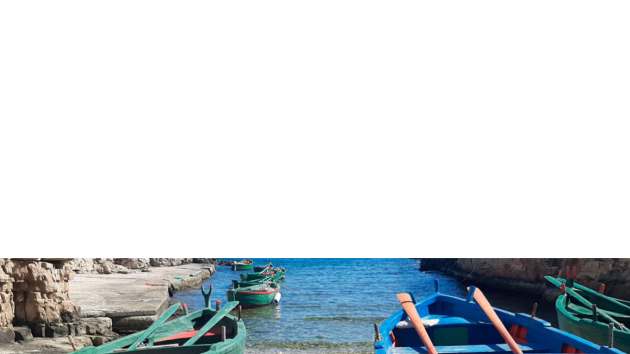
\includegraphics[width=\paperwidth]{background/template_169.pdf}}%
\begin{frame}[plain]
  \frametitle{\bf Deep Learning \& the Higgs Boson}
  \adjustbox{valign=t}{\begin{minipage}[t][0.55\textheight]{\linewidth}
      Classification with Fully Connected and Adversarial Networks.
      \vfill
      \begin{itemize}
      \item {\bf Lecture1: The Higgs boson and event classification:}\\
        - Event classification with a fully connected neural network (NN) with Keras API.\\
      \end{itemize}
      \vfill
      \begin{itemize}      
      \item {\bf Lecture2: Solving the background sculpting challenge:}\\
        - Event classification with adversarial neural network (ANN).\\
        - Hands-on knowledge of manipulating neural networks in Tensorflow.
      \end{itemize}
      \vfill
      \begin{itemize}          
      \item {\bf Lecture3: Putting it all together:}\\
        - Compare ANN classification performance to the fully connected network.
      \end{itemize}
      \vfill
\end{minipage}}
% vertical place-holder
\adjustbox{valign=t}{\begin{minipage}[t][0.35\textheight]{\linewidth} 
  \end{minipage}}
\end{frame}
}

\begin{frame}[plain]
  \frametitle{\bf Why is this useful?}
     \adjustbox{valign=c}{\begin{minipage}[c]{0.40\linewidth}   
         \begin{itemize}
         \item Classification with Adversarial neural network:
           generic solution for removing bias.
         \item \textcolor{EDBBlue}{Good tool for your toolbox.} 
         \end{itemize}
         \vspace{20pt}
         \begin{itemize}
         \item Research at LHC:\\ unique, big AI challenges.
         \item Bench-marking \& collaboration. 
         \item Image: \href{https://arxiv.org/abs/2201.08187v5}{\underline{LorentzNet}}, Microsoft.
         \end{itemize}         
     \end{minipage}}
     \hfill
     \adjustbox{valign=c}{\begin{minipage}[c]{0.59\linewidth}
         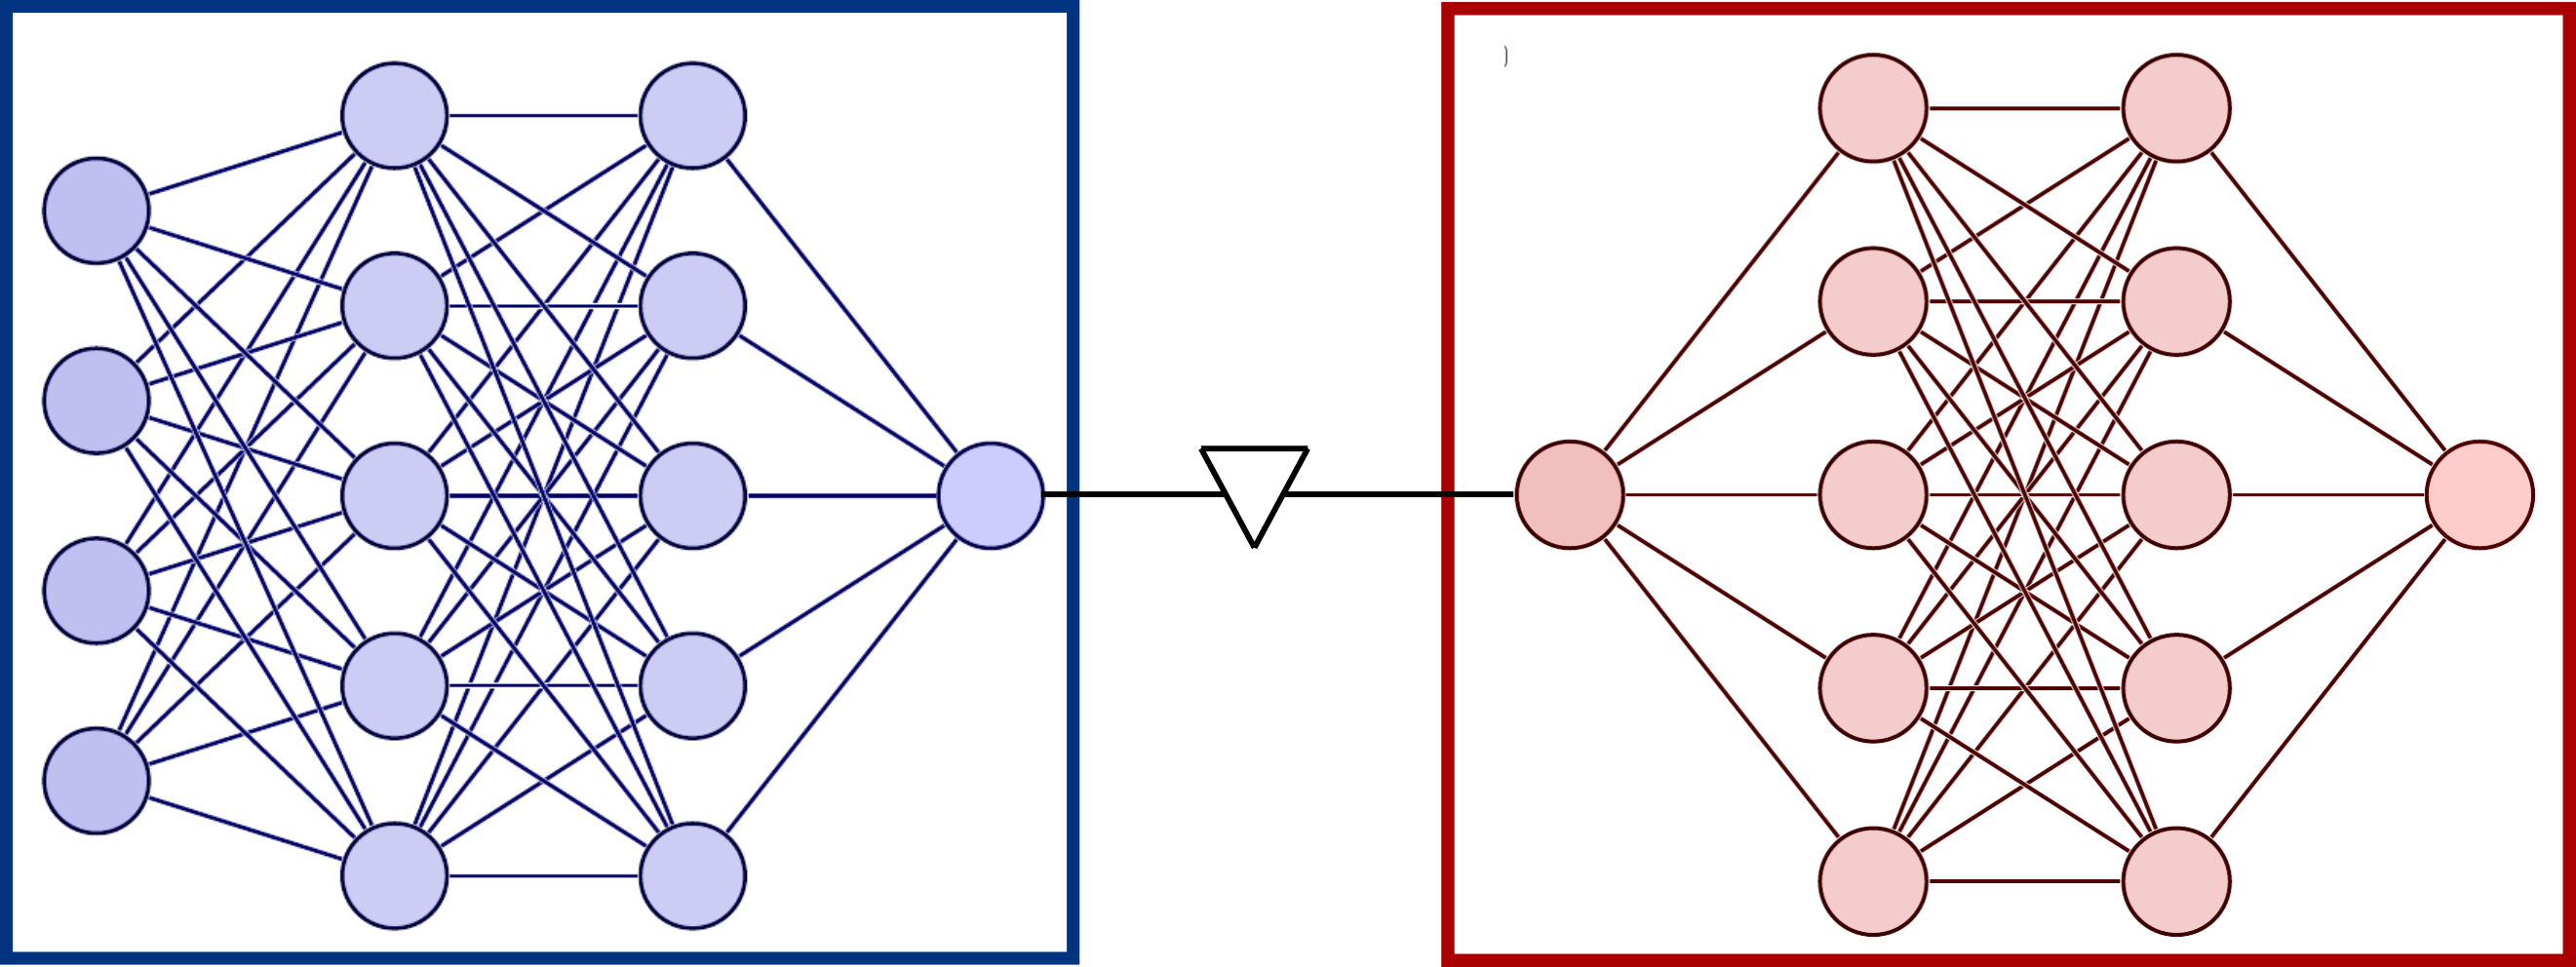
\includegraphics[width=1.00\textwidth]{figures/l1/intro/ann.png}
         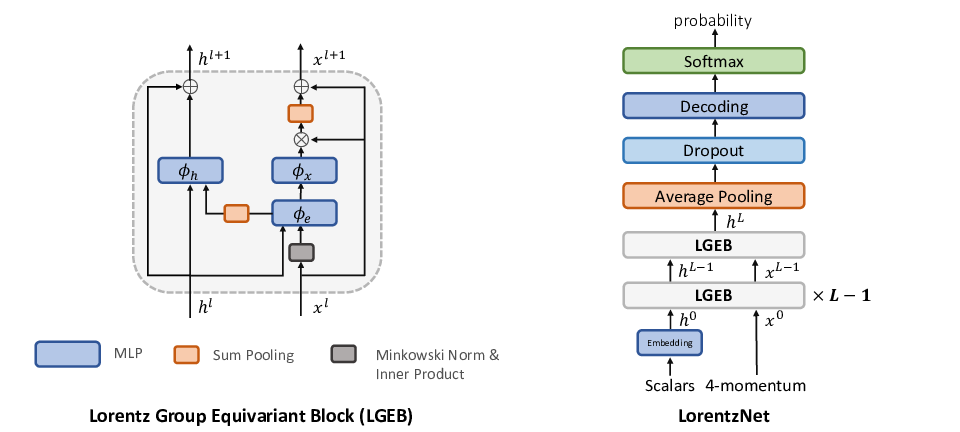
\includegraphics[width=1.00\textwidth]{figures/l1/intro/LorentzNet.png}
       \end{minipage}} 
 \end{frame}
 
\begin{frame}[plain]
  \frametitle{\bf Lecture Schedule}
     \adjustbox{valign=c}{\begin{minipage}[c]{0.6\linewidth}   
         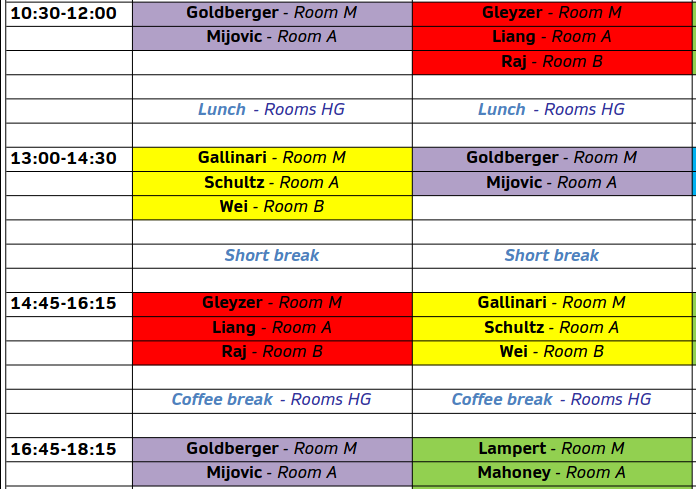
\includegraphics[width=1.00\textwidth]{figures/l1/schedule.png}
     \end{minipage}}
     \hfill
     \adjustbox{valign=c}{\begin{minipage}[c]{0.34\linewidth}
         {\bf Room A:}
         \vfill
          \begin{itemize}
            \item {\bf Lecture1: Mon Morning}
          \end{itemize}
          \begin{itemize}
            \item {\bf Lecture2: Mon Evening}
          \end{itemize}
          \begin{itemize}
            \item {\bf Lecture3: Tue Afternoon}
          \end{itemize}
          \vfill
          {\bf Please bring your laptop.}
     \end{minipage}}
\end{frame}


{
\usebackgroundtemplate{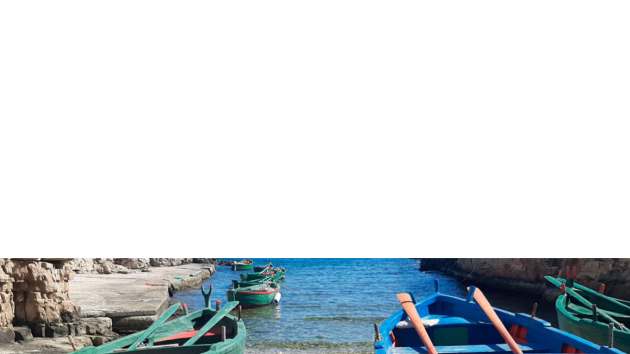
\includegraphics[width=\paperwidth]{background/template_169.pdf}}%
\begin{frame}[plain]
  \frametitle{}
  \adjustbox{valign=t}{\begin{minipage}[t][0.55\textheight]{\linewidth}
      \vfill
      \begin{center}
      {\bf \Huge Lecture1:\\[2ex] Higgs boson \& event classification:}\\[2ex]
        {\Large event classification with a fully connected neural network (NN) with Keras API.}\\
      \end{center}
      \vfill
\end{minipage}}
% vertical place-holder
\adjustbox{valign=t}{\begin{minipage}[t][0.35\textheight]{\linewidth} 
  \end{minipage}}
\end{frame}
}

\begin{frame}[fragile]
  \frametitle{\bf Fundamental Particles and Collisions}
  \begin{figure}
    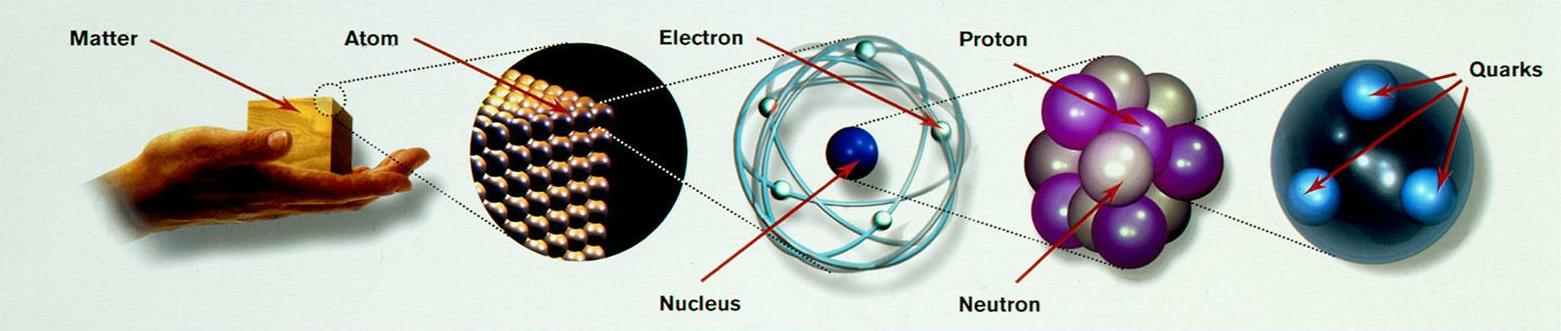
\includegraphics[width=1.0\textwidth]{figures/l1/intro/atom_to_quark.png}
  \end{figure}
  
  \adjustbox{valign=t}{\begin{minipage}[c]{0.5\linewidth} 
      \begin{figure}
        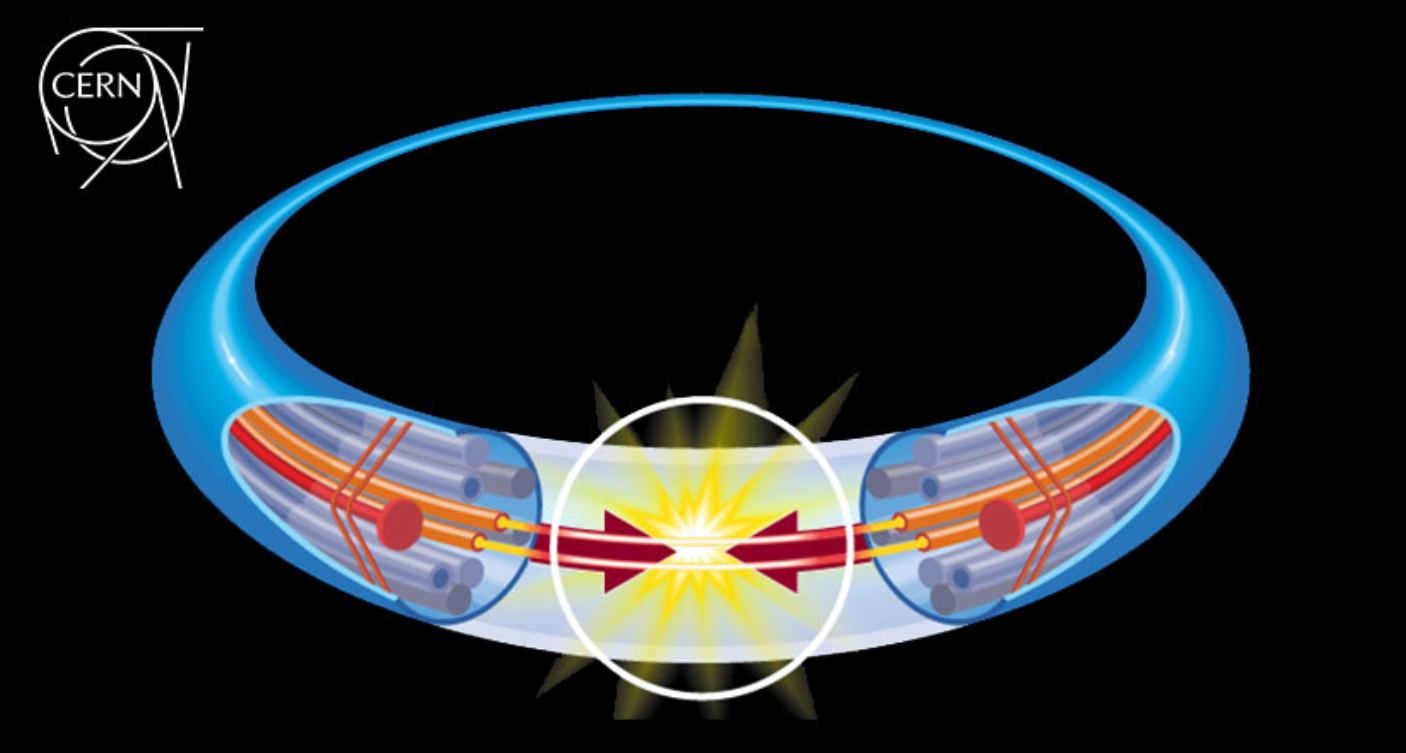
\includegraphics[width=1.00\textwidth]{figures/l1/intro/lhc_coll.png}
      \end{figure}
    \end{minipage}}
  \hfill
  \adjustbox{valign=t}{\begin{minipage}[c]{0.44\linewidth}
      \vspace{10pt}
      {\bf Large Hadron Collider (LHC):}
      \begin{itemize}
      \item {\bf Collide protons.}
      \end{itemize}
      \begin{itemize}
      \item {\bf New particles:} $\bm{\mathrm{E}} \bm{\sim} \bm{\mathrm{mc}}^{\bm 2}${\bf .}
      \end{itemize}
      \begin{itemize}
      \item {\bf Detector: snap-shot of collision.}
      \end{itemize}
    \end{minipage}} 
\end{frame}


\begin{frame}[fragile]
  \frametitle{\bf  Why study particle collisions?}
  % . Yet we know that the SM is not the ultimate theory. It
  \vspace{-5pt}
      \begin{figure}
        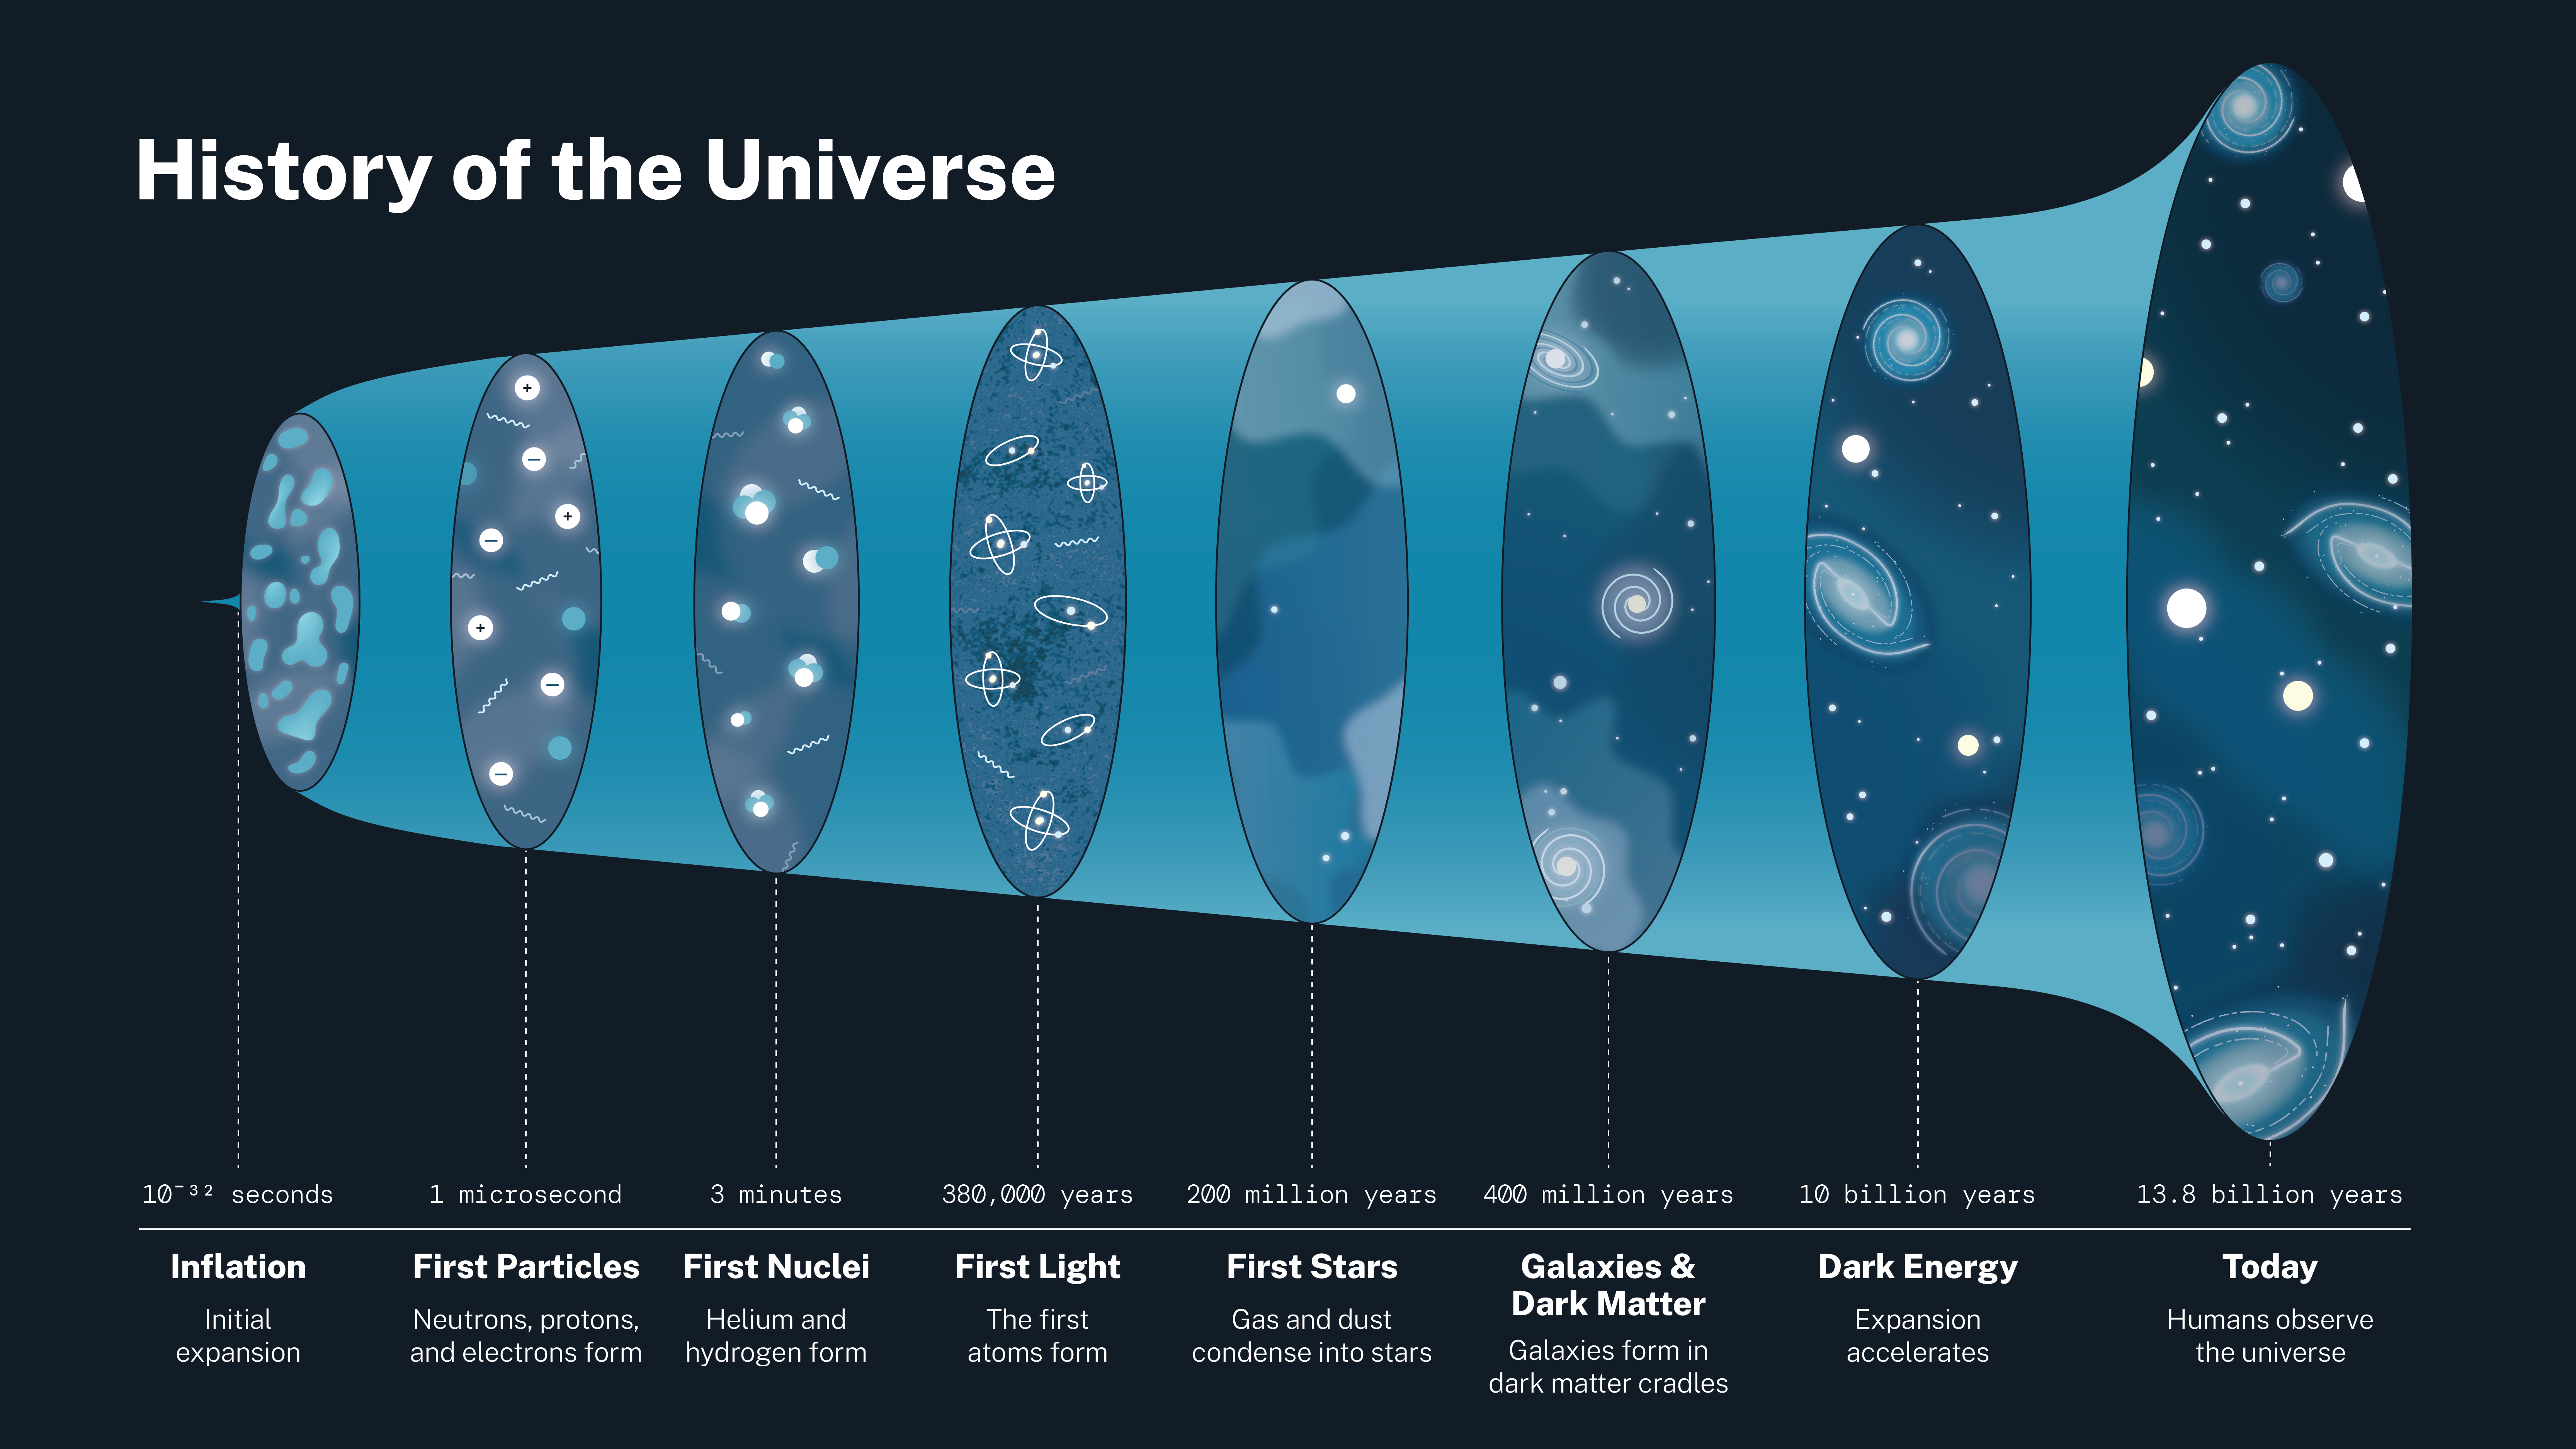
\includegraphics[width=0.85\textwidth]{figures/l1/intro/universe_nasa.png}
      \end{figure}
   \vspace{-5pt}   
      Cannot account for{$^*$}: dark matter, cosmic inflation, matter/anti-matter asymmetry. 
%      dark matter, cosmic inflation, matter/anti-matter asymmetry.
% neutrino masses,
%
%matter/anti-matter asymmetry, and , which are all experimental facts.
\blfootnote{Image
  credit: \href{https://universe.nasa.gov/universe/basics/}{NASA}.
  $^*$Additional observation we cannot account for are neutrino masses.}
    \end{frame}




\begin{frame}[fragile]
  \frametitle{\bf Challenge: Collisions are Complex}
    \adjustbox{valign=t}{\begin{minipage}[c]{0.5\linewidth} 
        \begin{figure}
          \centering
        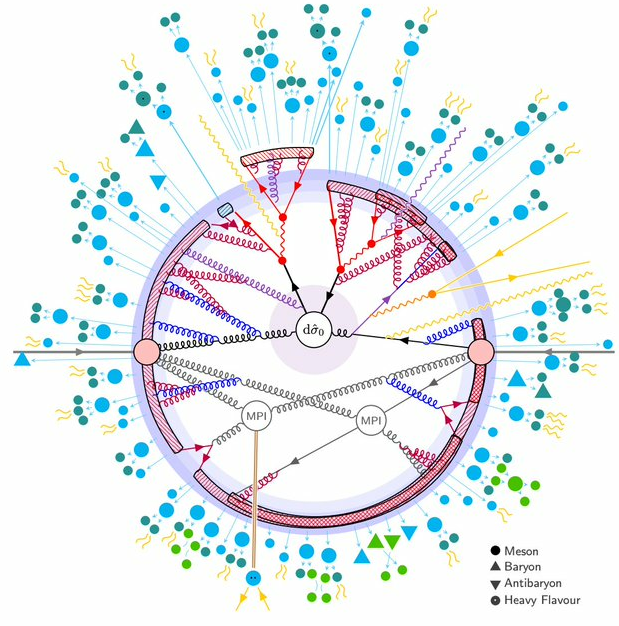
\includegraphics[width=1.00\textwidth]{figures/l1/intro/pp_nice.png}
      \end{figure}
      \end{minipage}}
    \adjustbox{valign=t}{\begin{minipage}[c]{0.49\linewidth}
      \begin{itemize}
      \item {\bf $\sim$ 1000 particles / collision.}
      \item {\bf Figure: inner-tracker.}
      \item {\bf 5B channels.}
      \end{itemize}
        
      \begin{figure}
        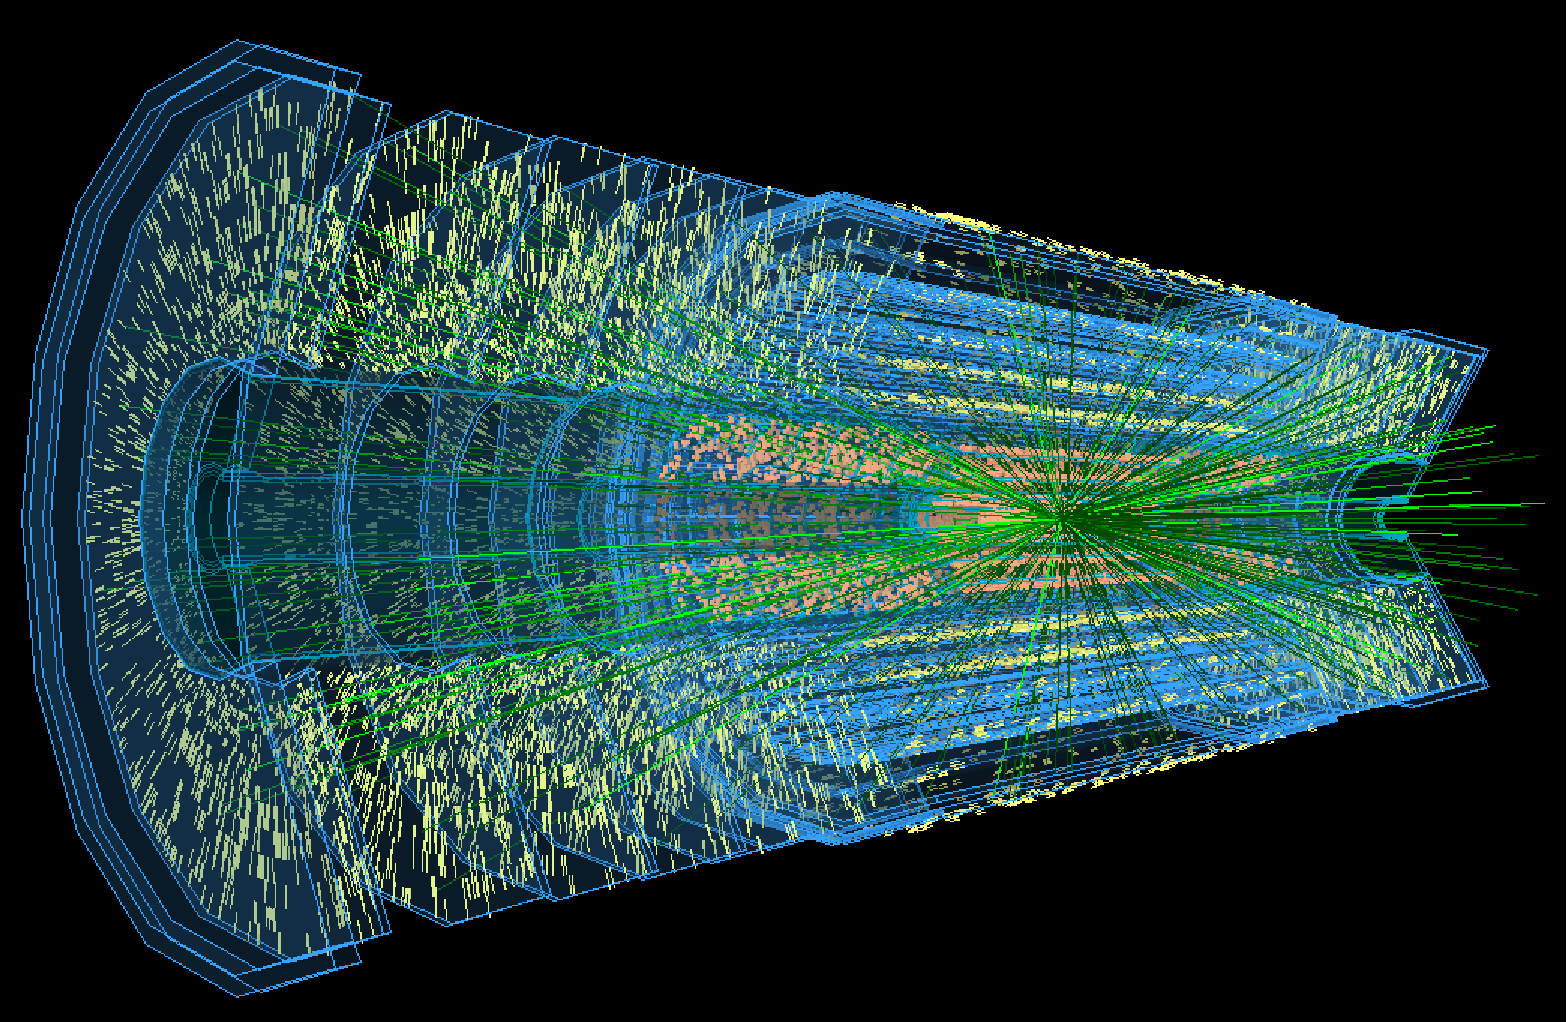
\includegraphics[width=1.00\textwidth]{figures/l1/intro/atlas-hl-lhc.png}
      \end{figure}

    \end{minipage}} 
\end{frame}

\begin{frame}[fragile]
  \frametitle{\bf LHC Detectors}
  \vspace{-5pt}
      \begin{figure}
        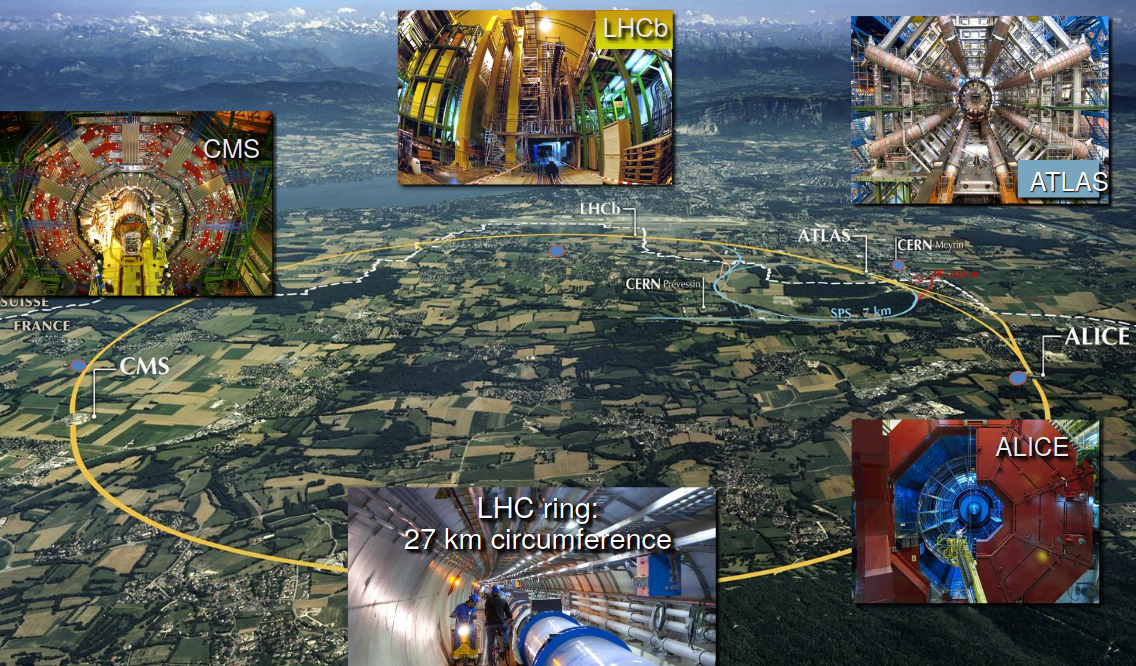
\includegraphics[width=0.90\textwidth]{figures/l1/intro/lhc_snip.png}
      \end{figure}
\end{frame}

\begin{frame}[fragile]
  \frametitle{\bf The Standard Model}
  \vspace{-5pt}
      \begin{figure}
        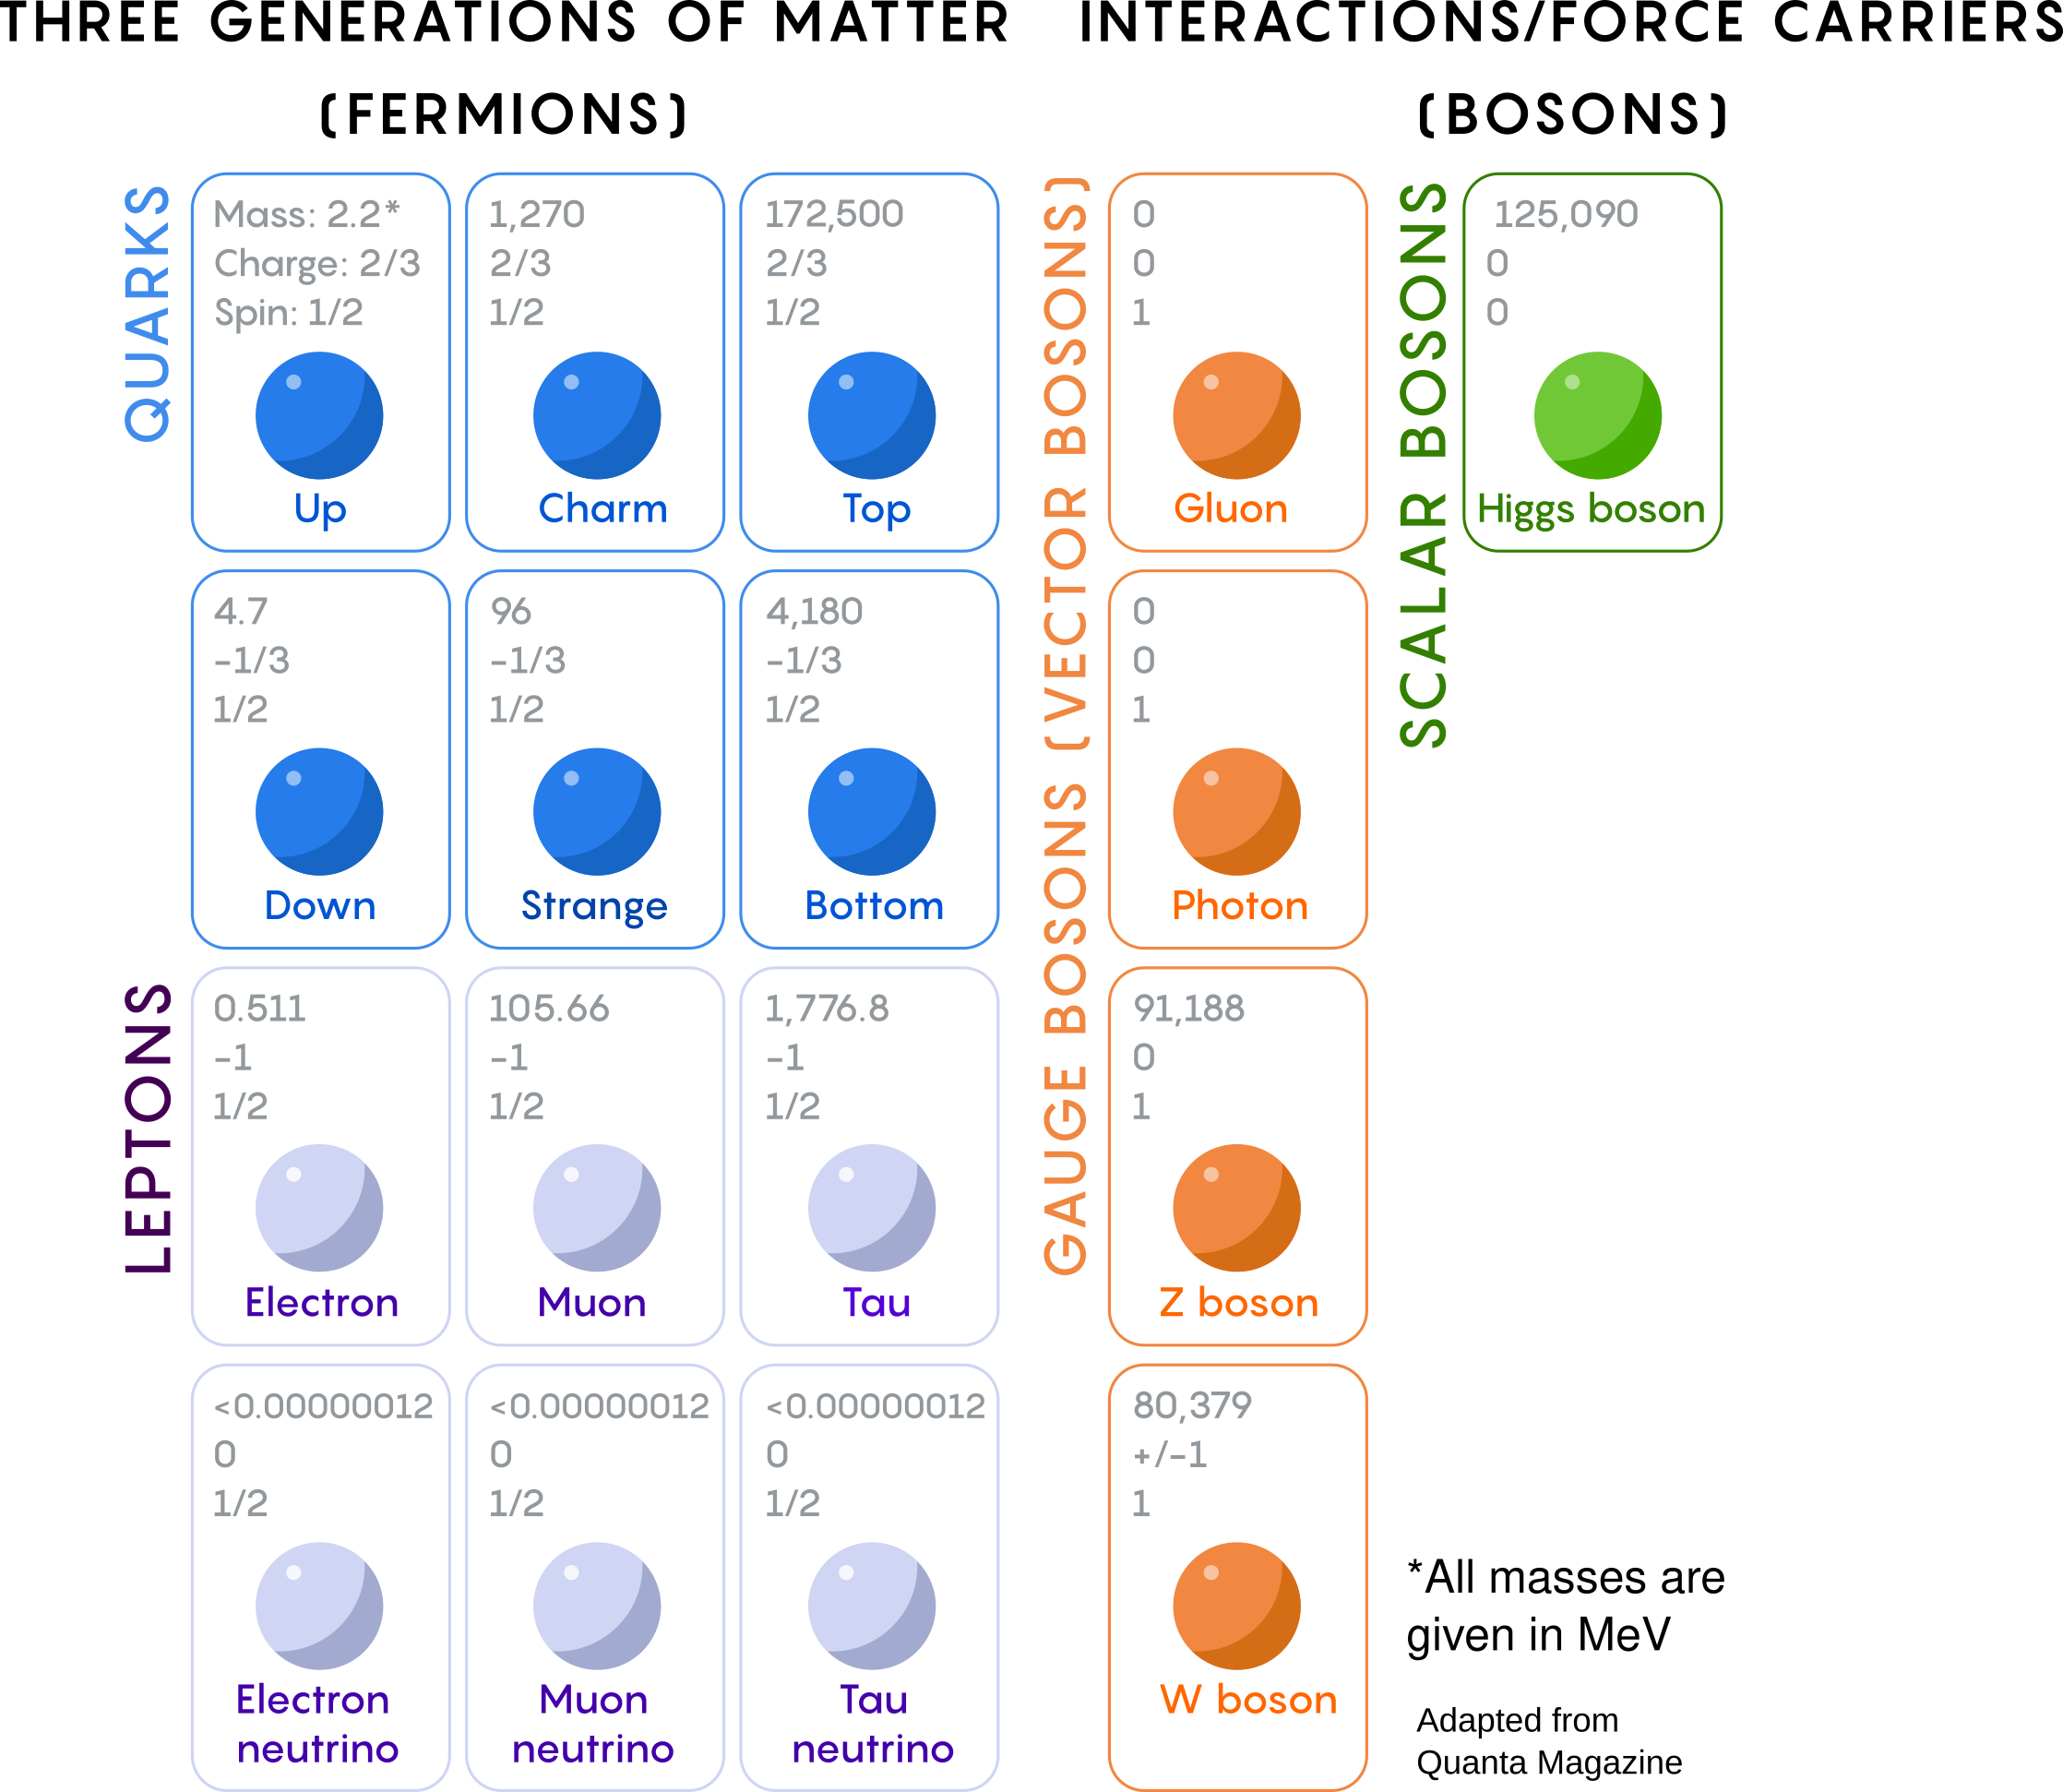
\includegraphics[width=0.60\textwidth]{figures/l1/intro/SM_qm_lm.png}
      \end{figure}
\end{frame}

\begin{frame}
  \frametitle{\bf The Higgs boson}
  \adjustbox{valign=c}{\begin{minipage}[t]{0.26\linewidth}
      \centering
      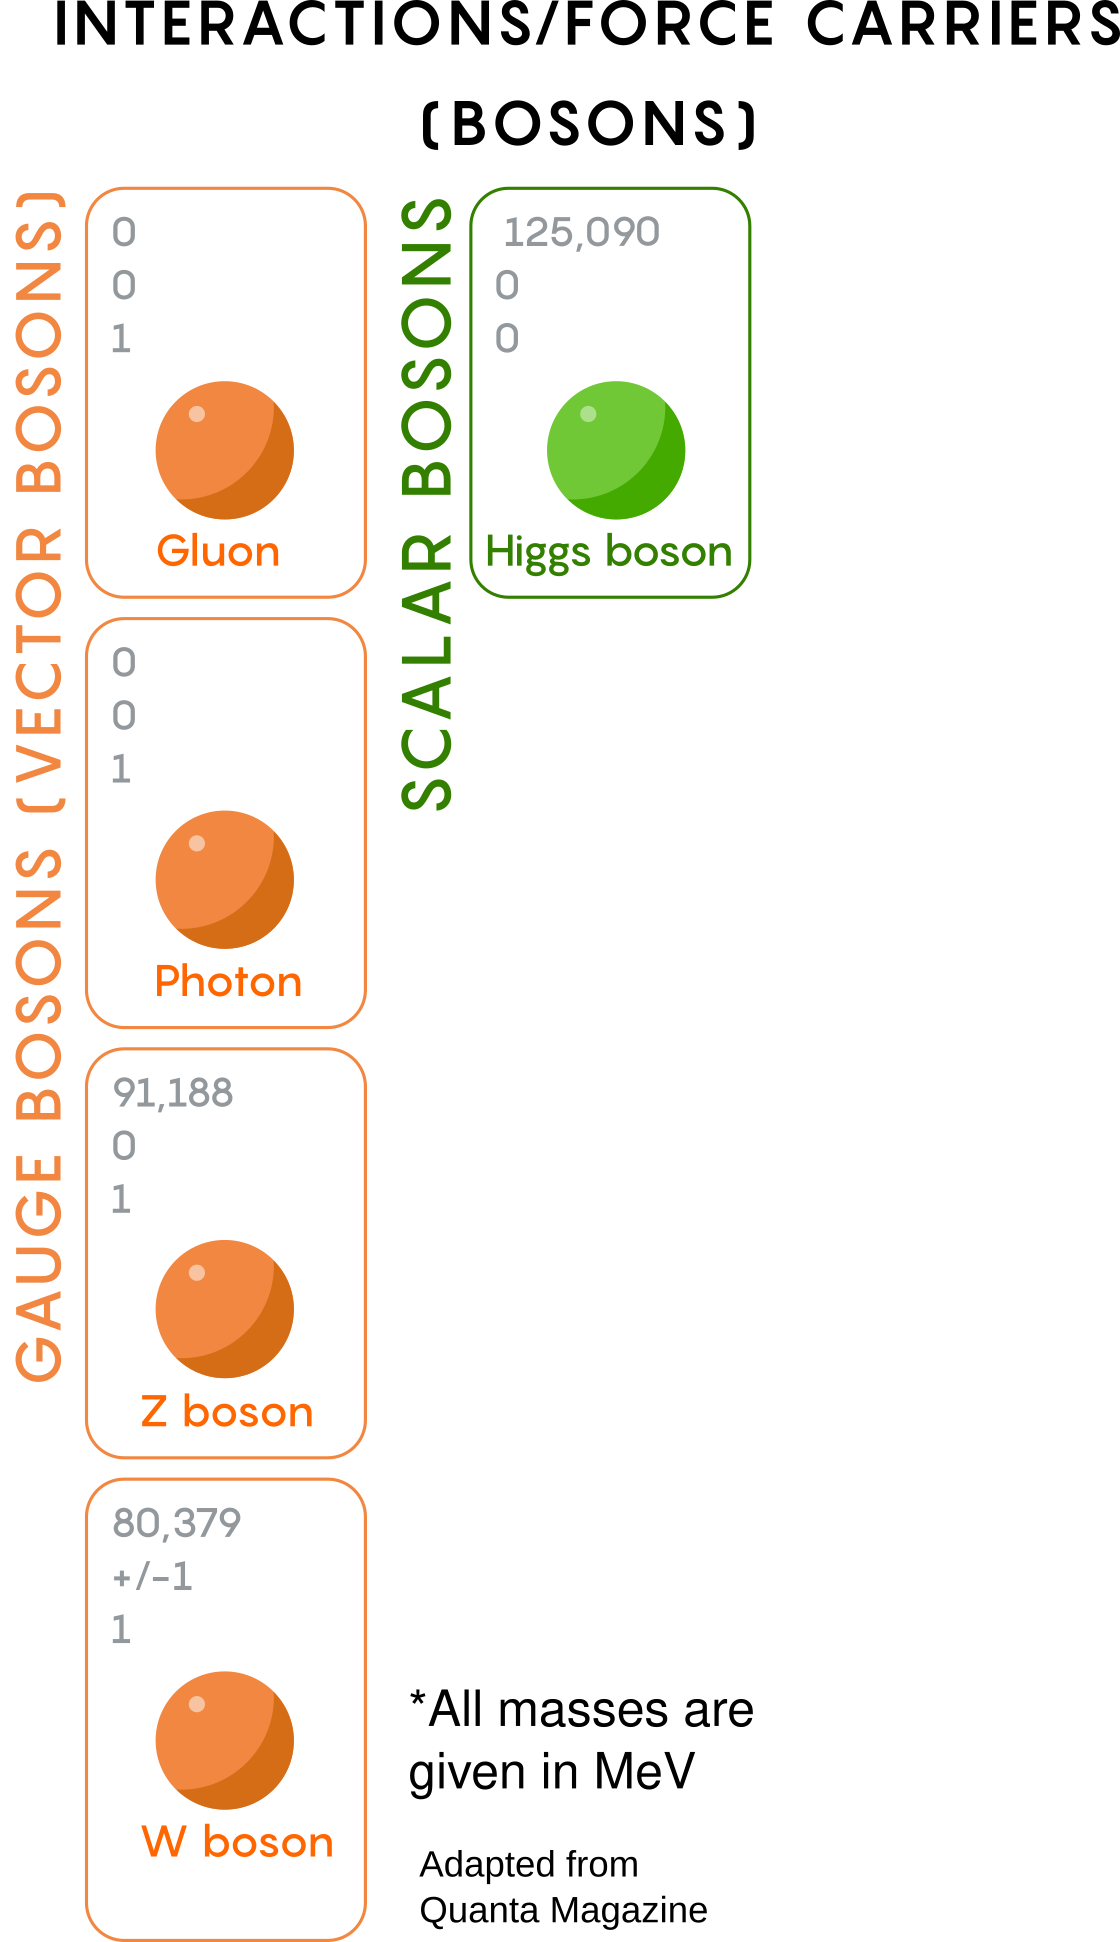
\includegraphics[width=0.98\textwidth]{figures/l1/intro/SM_qm_lm_bosons.png}
    \end{minipage}}\hfill
  \adjustbox{valign=c}{\begin{minipage}[t]{0.70\linewidth}
      \begin{itemize}
      \item 1964: R. Brout, F. Englert, P. Higgs:
        W, Z masses. 
      \item 2012: Higgs boson observation, ATLAS \& CMS
      \end{itemize}
      \hspace{0.1\textwidth}
      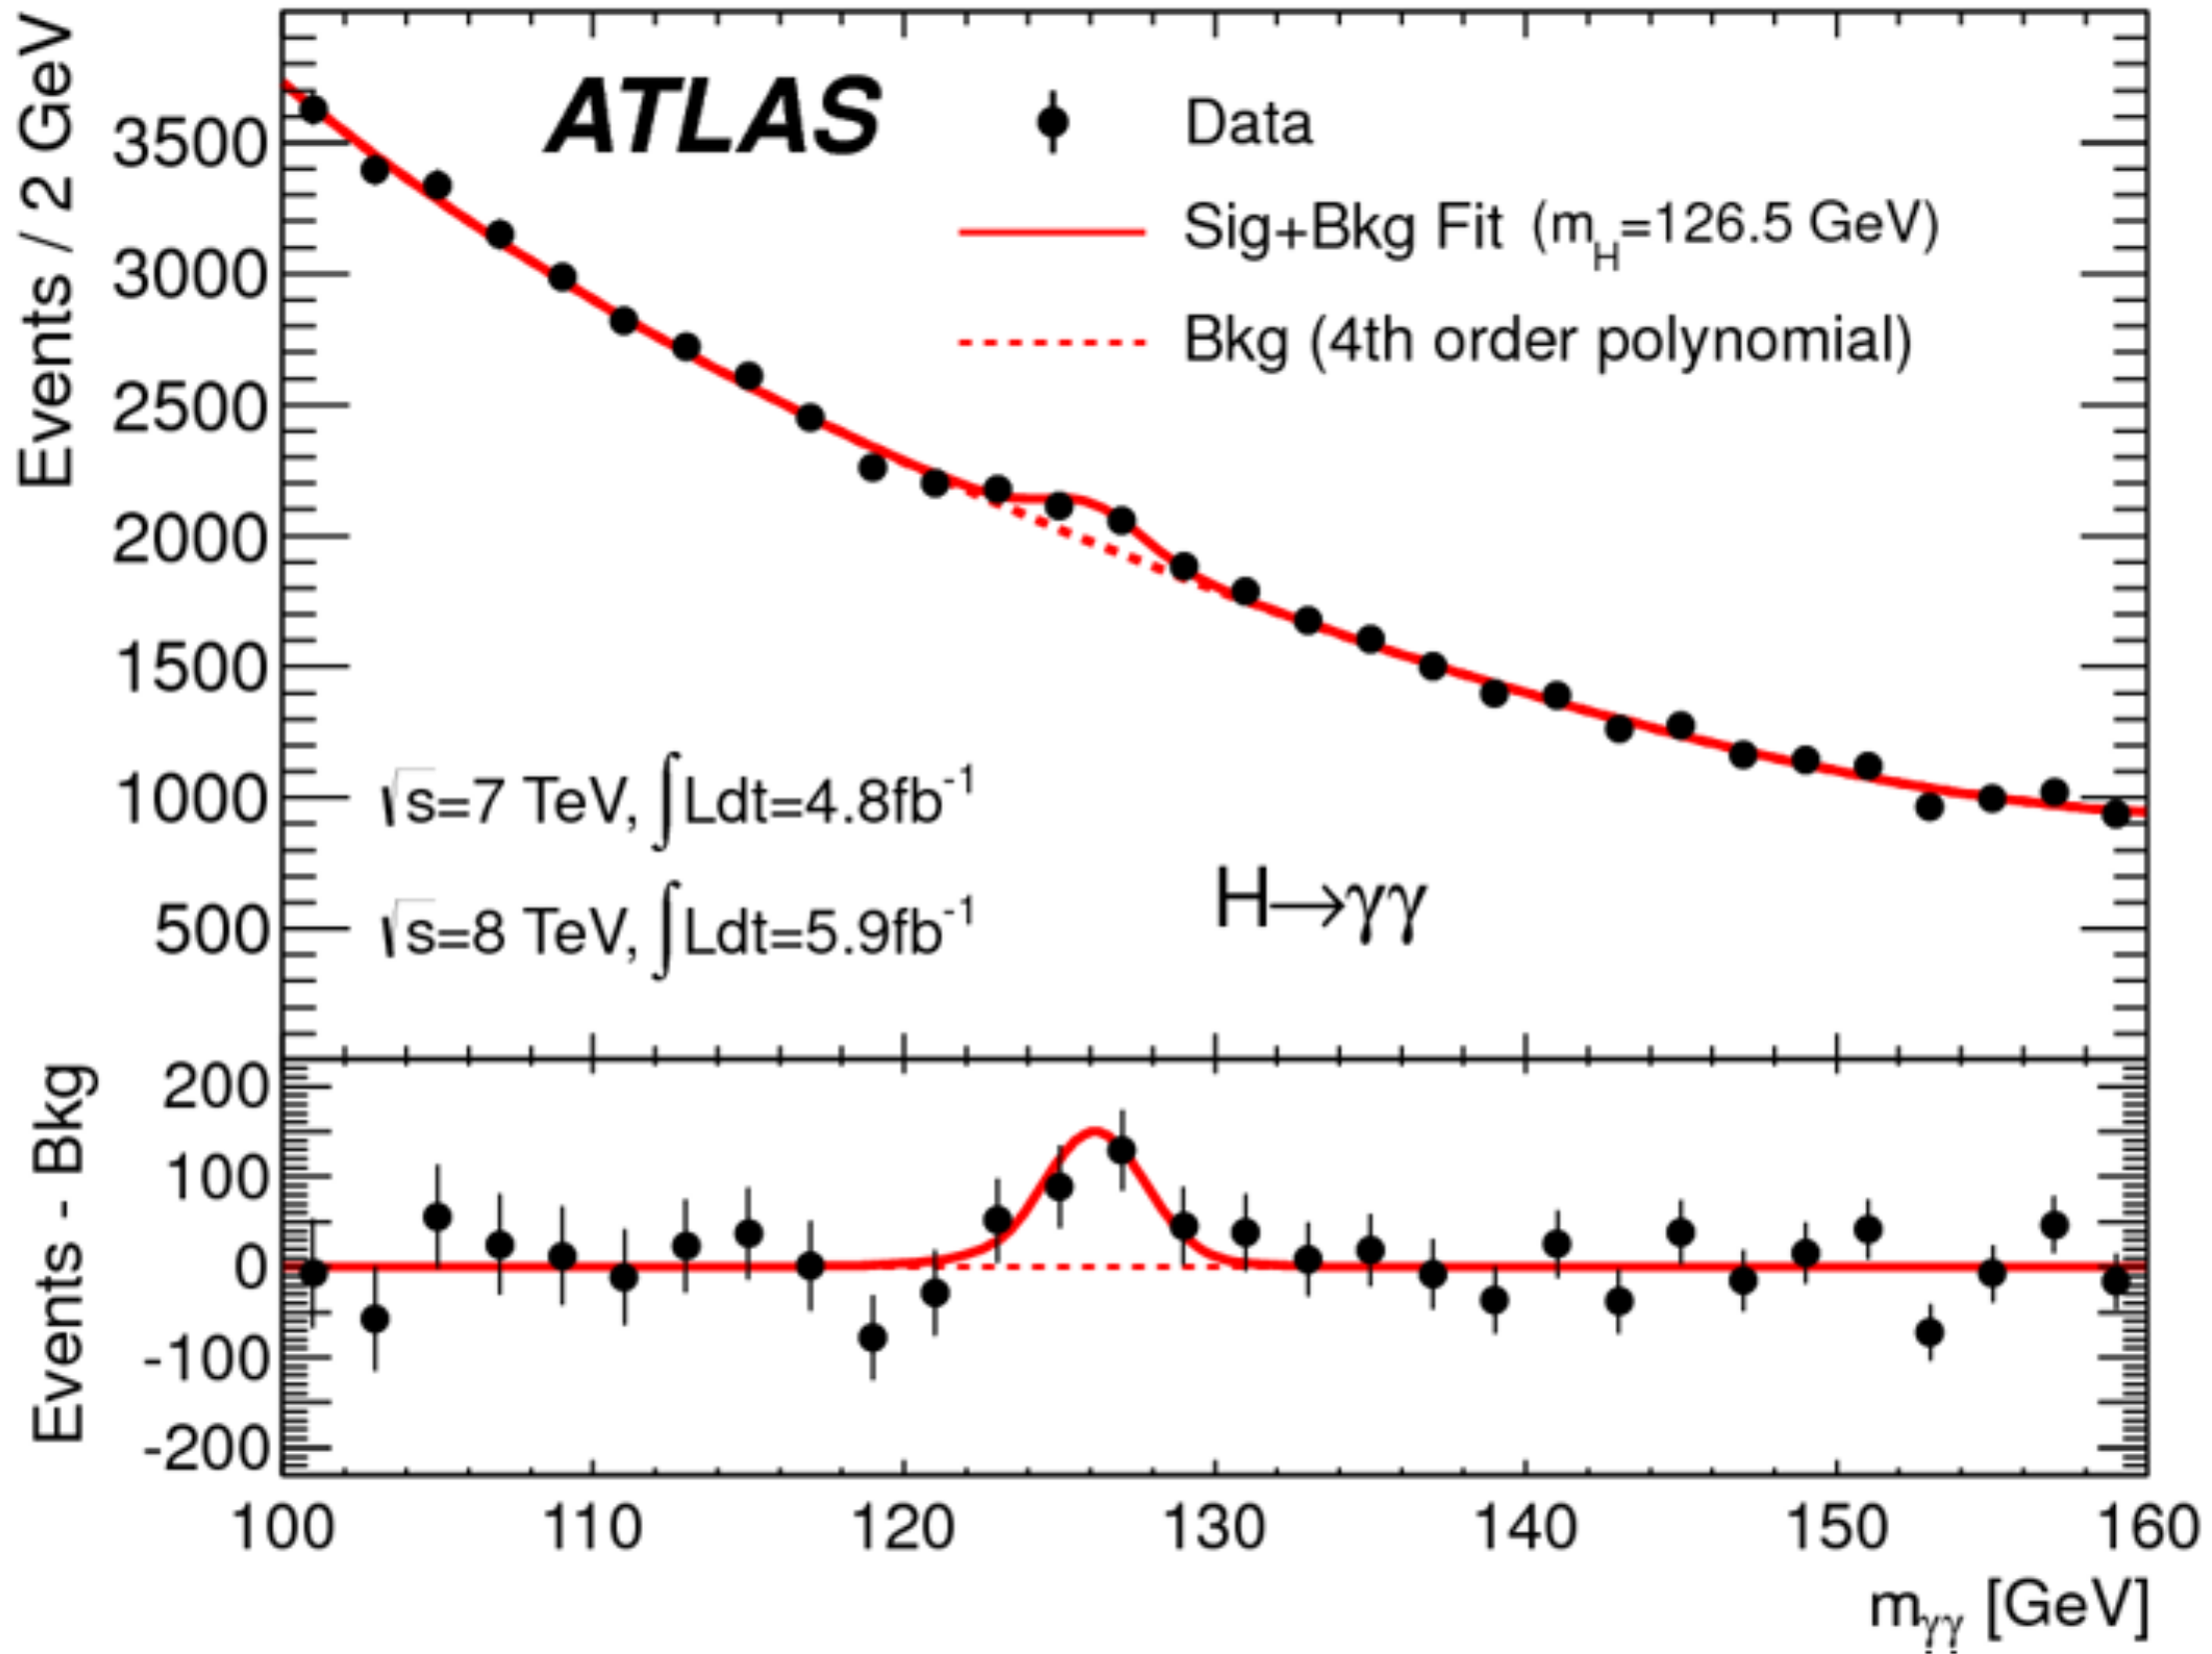
\includegraphics[width=0.6\textwidth]{figures/l1/intro/ATLAS_Higgs.png}
      \begin{itemize} 
      \item 2013: Nobel prize to F. Englert \& P. Higgs
      \end{itemize}      
    \end{minipage}}
\end{frame}


\begin{frame}
  \frametitle{\bf Our Challenge}

  \adjustbox{valign=t}{\begin{minipage}[c]{0.5\linewidth}
      \vfill
        {\bf Classification: separate}
        \begin{itemize}
        \item \textcolor{EDBRed}{Signal} with Higgs boson.
        \item \textcolor{EDBBlue}{Background} with no Higgs boson.
        \end{itemize}
        \vfill
        {\bf Approach:} 
        \begin{itemize}
        \item use synthetic data.
        \item \textcolor{Gray}{Introduce no bumps in the \myy{} distribution;
            these would hamper the background estimate.\\
            $\Rightarrow$ evening lecture.}
        \end{itemize} 
      \end{minipage}}
    \adjustbox{valign=t}{\begin{minipage}[c]{0.49\linewidth}     
      \begin{figure}
        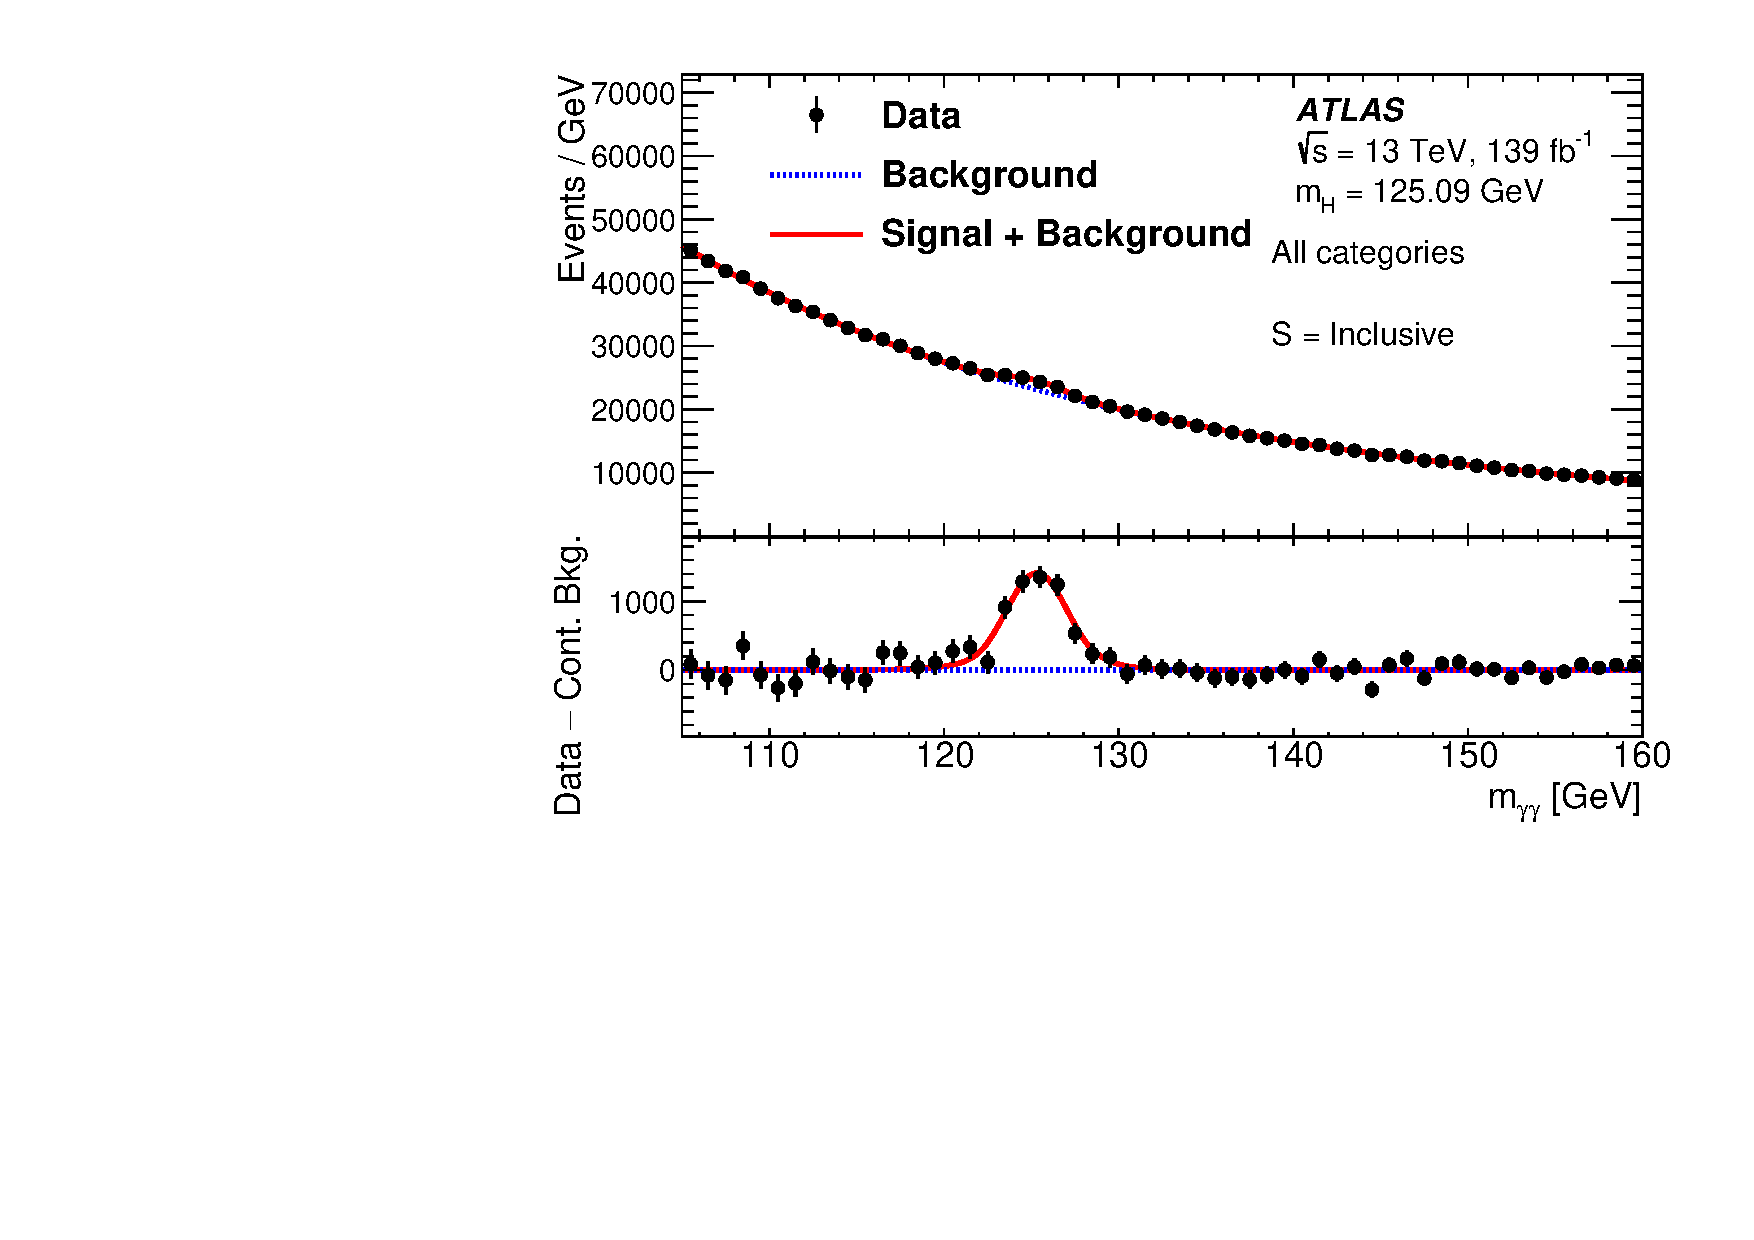
\includegraphics[width=1.00\textwidth]{figures/l1/challenge/figaux_01.pdf}
      \end{figure}
    \end{minipage}}
   \blfootnote{\scriptsize{L. Mijovi\'c, ATLAS, \href{https://arxiv.org/abs/2207.00348}{JHEP (2022)}.}}  
\end{frame}


\begin{frame}
  \frametitle{\bf What is in the data?}
  \begin{center}
    Two photons ($\gamma$) per event, with momenta $p$.\\
    \vspace{20pt}
  \textcolor{EDBRed}{\Large Signal, label=1} \hspace{0.25\textwidth}
  \textcolor{Blue}{\Large Background, label=0}
  \end{center}
      \begin{figure}
        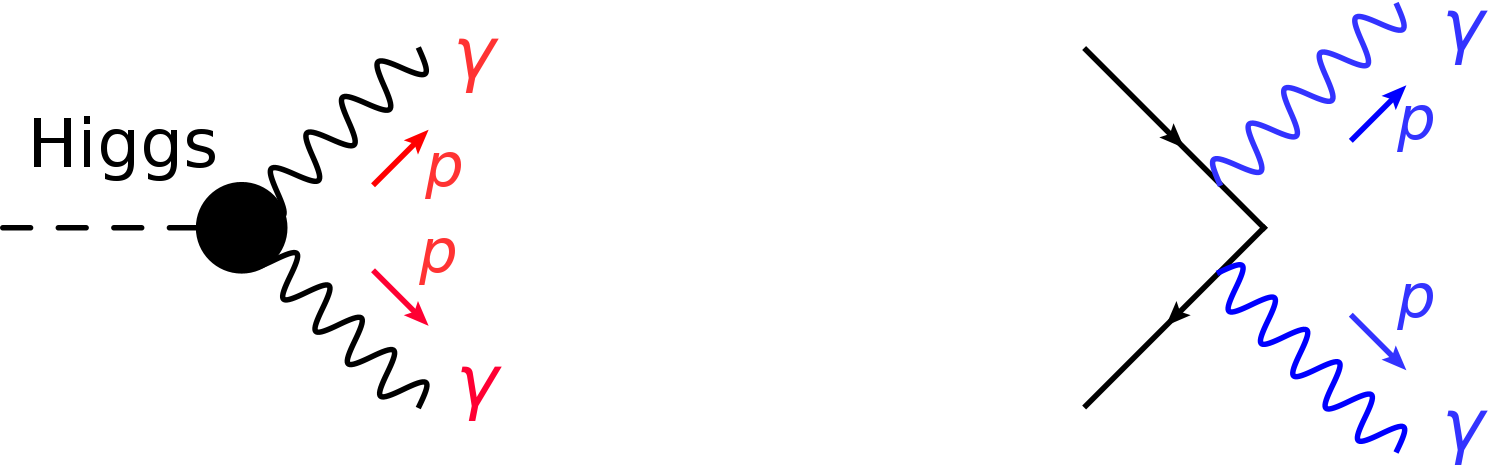
\includegraphics[width=0.80\textwidth]{figures/l1/challenge/SvsB.png}
      \end{figure}     
\end{frame}

\begin{frame}
  \frametitle{\bf What is in the data?}
  Momenta $p$ have two catches:
  \vfill
  \begin{itemize}
  \item (1) They are 4-dimensional (Lorentz) vectors.
  \end{itemize}
  \begin{figure}
    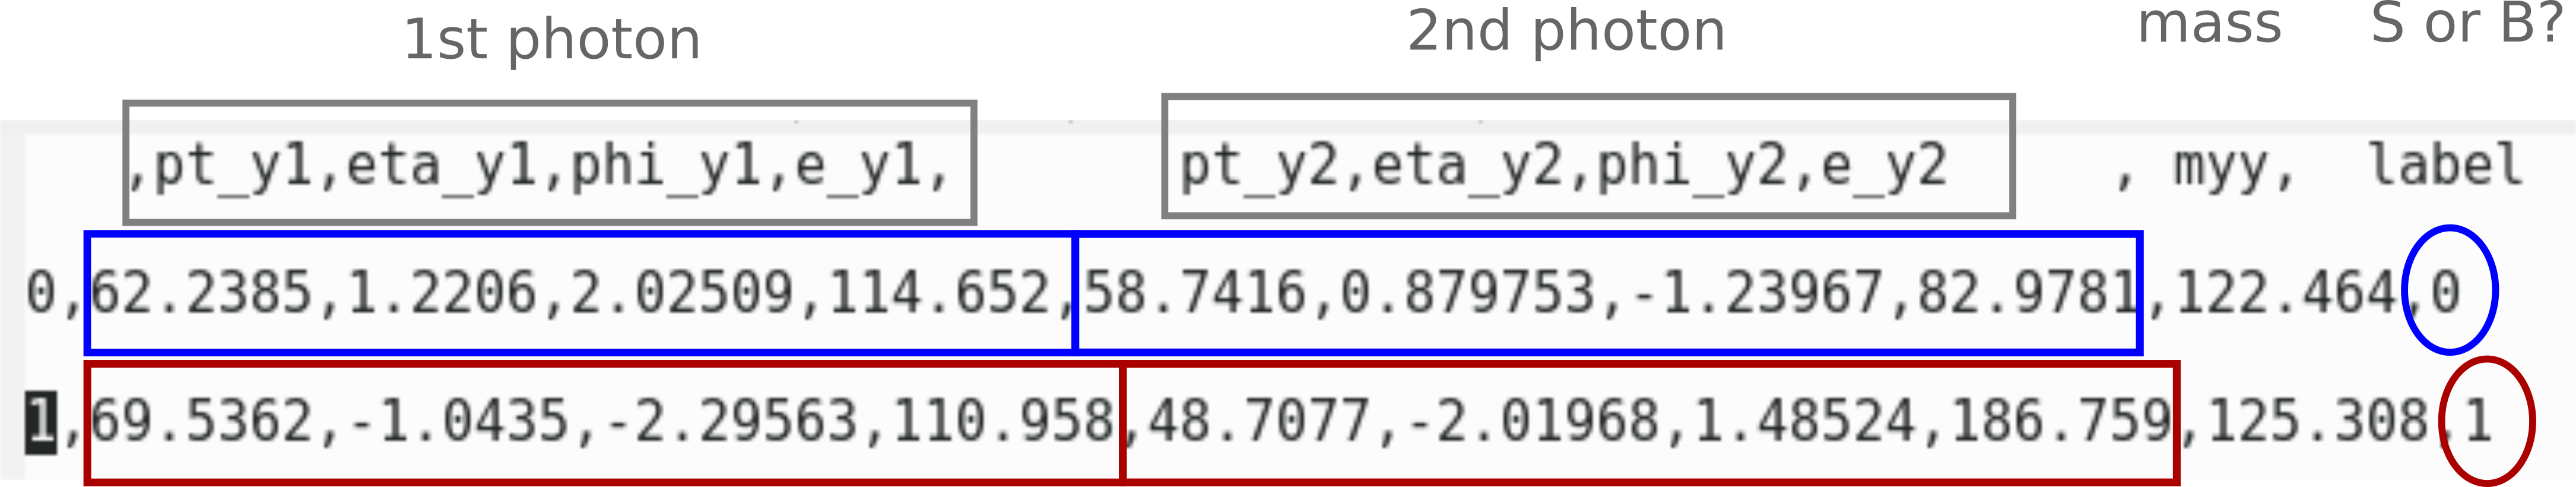
\includegraphics[width=1.00\textwidth]{figures/l1/challenge/data_annot.png}
  \end{figure}
\end{frame}

\begin{frame}
  \frametitle{\bf What is in the data?}
  Momenta $p$ have two catches:
  \vfill
  \begin{itemize}    
  \item (2) They are passed in cylindrical coordinates.
  \end{itemize}
  \begin{figure}
    \centering
    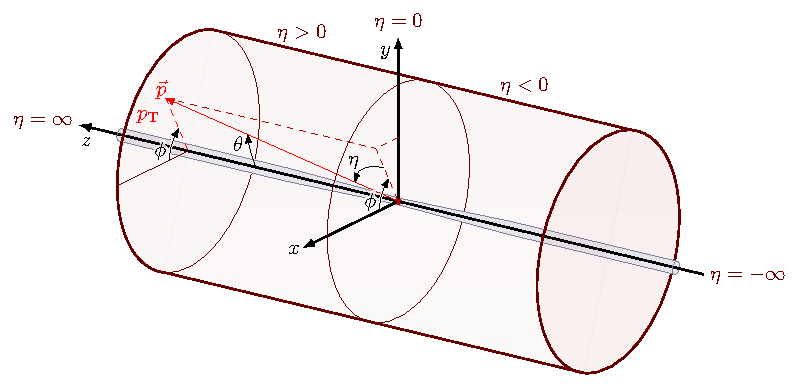
\includegraphics[width=0.80\textwidth]{figures/l1/challenge/coordinate_system.pdf}
  \end{figure}
\blfootnote{Image: \href{https://tikz.net/axis3d_cms/}{adapted from I.
    Neutelings}, CC BY-SA 4.0}
\end{frame}

\begin{frame}
  \frametitle{\bf Hands-on work}

  {\bf Let's get set up!}
  \begin{itemize}
  \item Download the data: \href{https://cern.ch/dl23data}{\textcolor{EDBBlue}{https://cern.ch/dl23data}}
  \item Set up the environment: \href{https://cern.ch/dl23code}{\textcolor{EDBBlue}{https://cern.ch/dl23code}}
  \end{itemize}
  \vfill
  {\bf Let's do some classification!}\\
  Using data\_scaled\_200k.csv try to classify signal vs background. 
  \begin{itemize}
  \item Use Keras \& fully connected deep neural network.
  \item Use photon momenta as (8) input features.
  \item Do not use myy as input feature.
  \end{itemize}
  {\bf Let's share resuts:}
  \begin{itemize}
  \item \href{https://cern.ch/dl23lect1}{\textcolor{EDBBlue}{https://cern.ch/dl23lect1}}
  \item Classification performance, eg ROC curve, accuracy etc.
  \item S and B myy distribution, for high discriminant scores (events likely to
    be S). 
  \end{itemize}
\end{frame}


\backupbegin

{
\usebackgroundtemplate{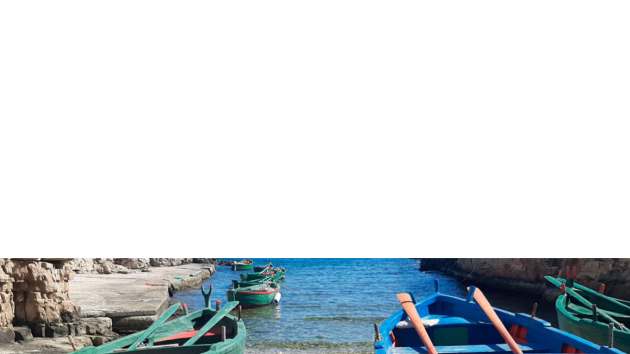
\includegraphics[width=\paperwidth]{background/template_169.pdf}}%
\begin{frame}[plain]
  \begin{center}
    \setlength{\parskip}{0pt}
    \vspace{10pt}
    {\Huge\bf Extra}
  \end{center}
\end{frame}
}

{
\usebackgroundtemplate{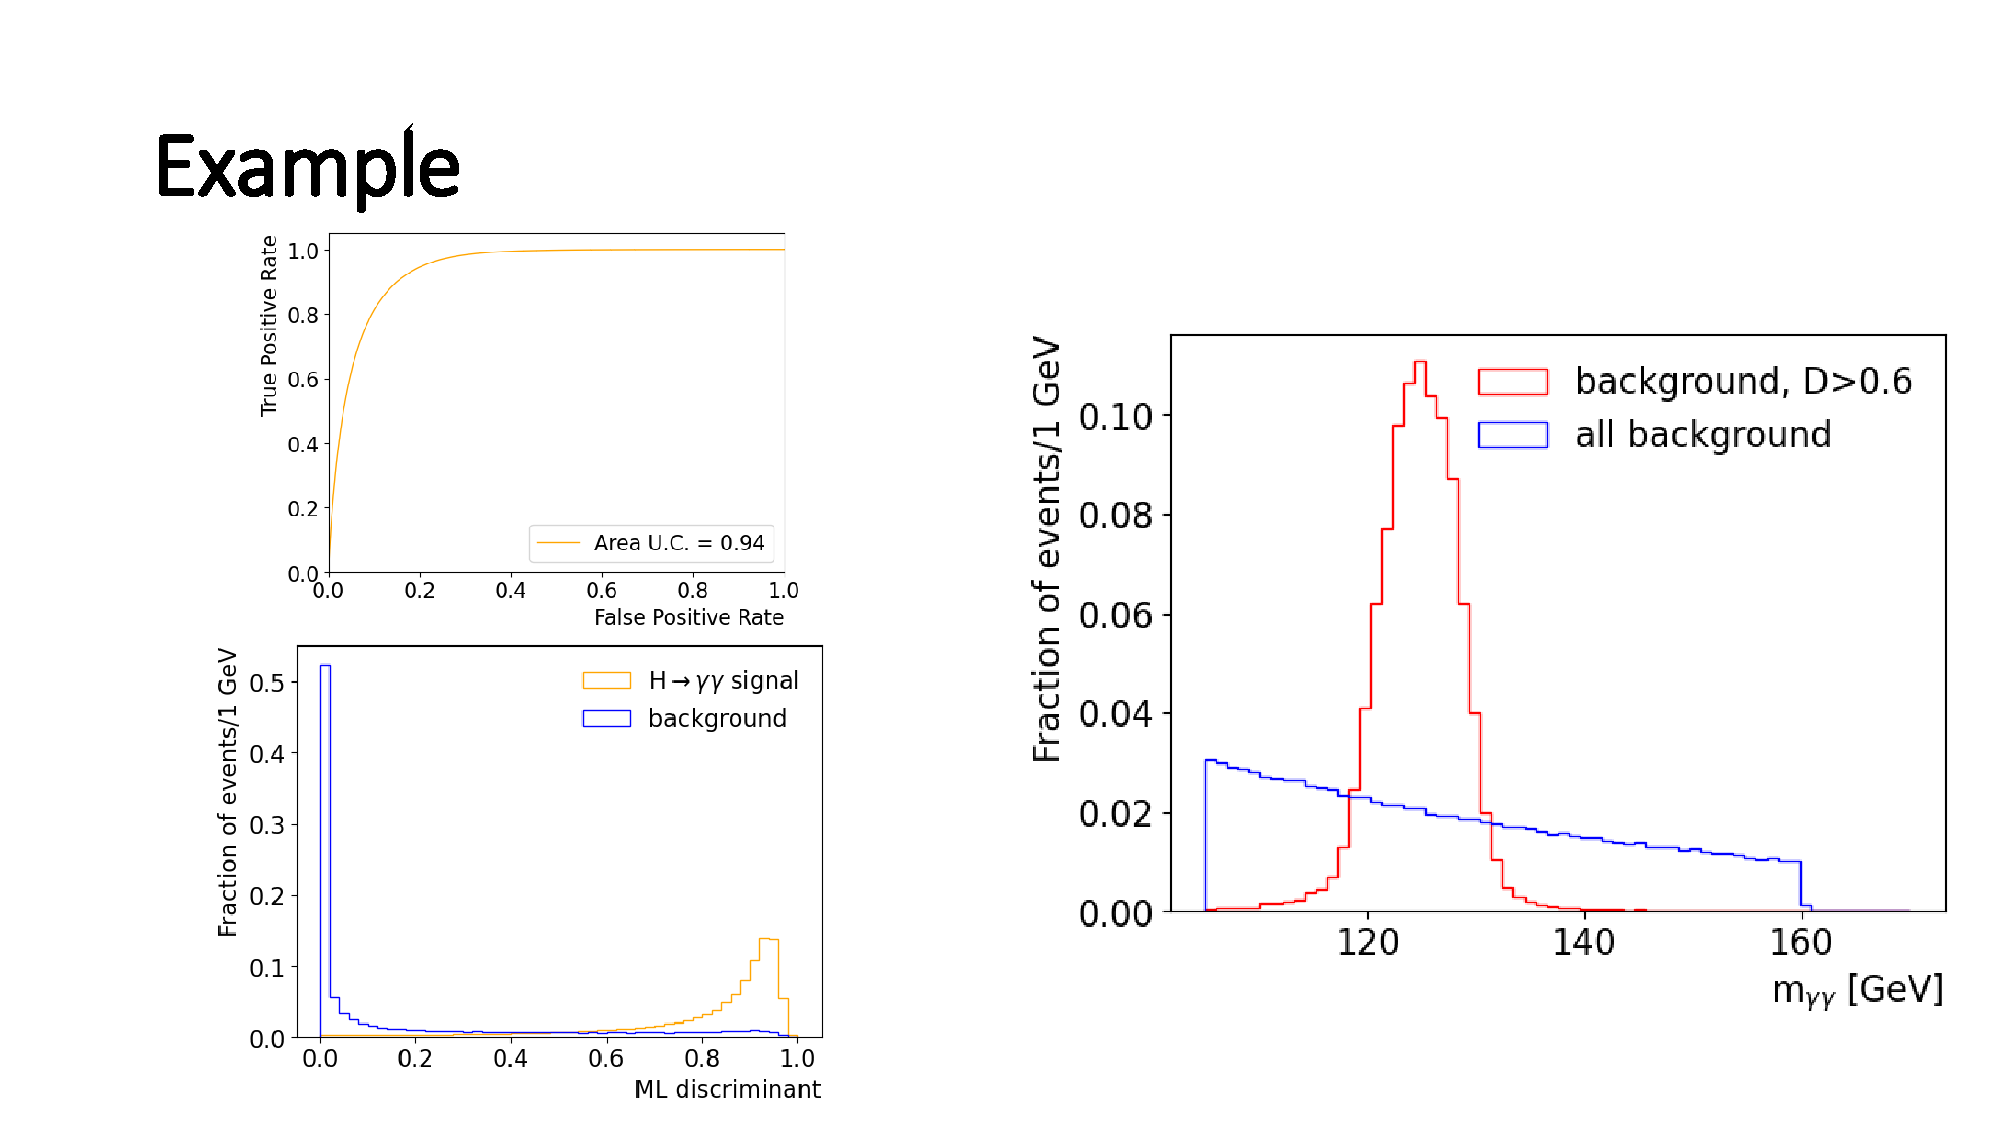
\includegraphics[width=\paperwidth]{figures/l1/challenge/example_share}}%
\begin{frame}[plain]
\end{frame}
}
\backupend

\end{document}
